\documentclass{article}
\usepackage[utf8]{inputenc}
\usepackage{listings}
\usepackage{graphicx}
\usepackage{float}
\usepackage{xcolor}
\usepackage{geometry}
\usepackage{CJKutf8}

\geometry{a4paper,scale=0.8}
\lstset{
    basicstyle          =   \sffamily,        
    keywordstyle        =   \bfseries,         
    commentstyle        =   \rmfamily\itshape, 
    stringstyle         =   \ttfamily, 
    flexiblecolumns,               
    numbers             =   left,  
    showspaces          =   false, 
    showstringspaces    =   false,
    captionpos          =   t,     
    frame               =   lrtb, 
}

\lstdefinestyle{Python}{
    language        =   Python, % 语言选Python
    basicstyle      =   \zihao{-5}\ttfamily,
    numberstyle     =   \zihao{-5}\ttfamily,
    keywordstyle    =   \color{blue},
    keywordstyle    =   [2] \color{teal},
    stringstyle     =   \color{magenta},
    commentstyle    =   \color{red}\ttfamily,
    breaklines      =   true,  
    columns         =   fixed,  
    basewidth       =   0.5em,
}

\title{\bf\Large  概率论与数理统计 第1次作业}
%%%%%%%%%%%%%%%%%%%%%%%%%%%%%%%%%%%%%%
%% DON'T forget to change this part %%
\author{\bf Name: 宋昊原 \qquad Student ID: 2022010755}
%%%%%%%%%%%%%%%%%%%%%%%%%%%%%%%%%%%%%%

\begin{document}
\begin{CJK}{UTF8}{gbsn}
\maketitle

\section{概率发展史}
概率发展史主要分为三个阶段:古希腊时期,哲学家们建立了朴素的概率观念;17至18世纪,Pascal和Fermat的通信奠定了概率论基础,而Bernoulli研究的二项分布等为概率进一步赋予了实用价值;19至20世纪,以Laplace和Kolmogrov为主的数学家奠定了概率论的公理化基础.\\
\par我认为,很多数学的分支学科都有着类似的发展规律,从朴素观念的建立,到深入发展理论以应用到生产生活和科学研究,再到建立严格的理论体系. 至少对于微积分、代数等学科也是如此. 
\\\par这同时也为我们学习数学建立了方法论的指导:我们在学习一个数学的分支学科时,第一步是建立一个朴素的感知,例如概率是对于可能性的描述,这一点在小学阶段甚至更早就已经有所认识;第二步是学习其富有应用意义的讨论,例如各种离散的或连续的概率分布,这一点在高中有所涉及,在大学课程中将会进一步讨论;第三步是理解其理论基础,例如概率论的公理化体系,从而对这个学科有更深刻的理解和应用,这一点更是大学课程需要完成的飞跃. 以上是我对概率发展史和大学概率论学习的主要理解.
\section{Bertrand悖论}
Bertrand悖论是下述问题:
\par在圆内随机取一条弦,这条弦的长度比圆内接三角形的长的概率是多少?
\par这个问题有不同的“随机选取”方法,比如:(a)随机选择两个点相连得弦;(b)随机选择一条半径和上面的随机一个点作垂直弦;(c)随机选择圆内一点,以之作为中点作弦.
\par根据不同的方法,所求的概率会有很大差异,例如(a)$\frac{1}{3}$,(b)$\frac{1}{2}$,(c)$\frac{1}{4}$.
\par且如果按照一些其他的方法,概率也不敢保证会相同.
\\
\par显然,这个问题的主要原因是,“随机选择一条弦”是一个没有良定义的过程. 我认为其主要原因是,一条弦并非是一个有单一自由度的选择(单一自由度指例如在一条线段上随机取一个点,这个点总是可以由其坐标唯一确定,且这是绝对最优的“随机选择”方式),然而对于一条“随机弦”,我们可以用很多不同的维度描述它,例如(a)两个端点,(b)垂径和垂径上的垂足位置,(c)中点位置. 这些确定弦的依据很难比较孰优孰劣,在不同的案例中有不同的答案.
\par类似的对于“随机选取”不良定义的问题我之前还有思考过另一个案例,与Bertrand悖论并不完全一样. 我曾听过一个结论:“在数轴上任取一个点,取到有理数的概率是0”. 这个看上去很有道理,但我总认为“在数轴上任取一个点”是一件很难进行良定义的事情. 如果我们将“任意”理解为数轴上任意一块的概率密度相同,那么会导致每一部分的概率密度都是0. 这实际代表着,无论我们取多大的有限的次数,这些样本的绝对值总是有界的,在这个界限之外的位置在这些次数中被取到的频率是0. 这显然对我们对于“在整个数轴上任意选取”的期望不符合. 因此我认为这种选取似乎也是不良定义的.
\par也许,上面那个命题的意思是“在数轴上的一条线段上任意选取一点,选到有理数的概率是0”,这便可以解释,毕竟无理数的数量($\aleph_{1}$)远远大于有理数的数量($\aleph_{0}$).
\par生活中不良定义的“随机”似乎还有很多,因此,建立概率的公理化体系是必要的.

\section{奖金分配}
两人水平相当,可假设每一局二人获胜的概率均分别为$\frac{1}{2}$,则乙获胜的概率为
$$ \frac{1}{2} \times \frac{1}{2} = \frac{1}{4} $$
甲获胜的概率为
$$ 1 - \frac{1}{4} = \frac{3}{4} $$
按照两人此时的奖金期望来分配,则甲得
$$ 200\times\frac{3}{4}=150 $$
元.
\\\\
乙得
$$ 200\times\frac{1}{4}=50 $$
元.
\section{两队对赌}
设A队获胜概率为$p$,则此人净收益期望
$$ E=5p-20(1-p) $$
设此净收益期望非负(既然愿意这样赌应当至少遵循了这样的原则),则有
$$ 5p-20(1-p)\geq0$$
解得
$$ p\geq\frac{4}{5} $$
即A队获胜的主观概率至少是$\frac{4}{5}$.
\section{三马下注}
设下注给A、B、C三匹马的获胜收益率(这里定义为总收入与投入金额之比)分别为$w_{A}$、$w_{B}$、$w_{C}$,则有
$$ w_{A}=\frac{1000}{500}=2 $$
$$ w_{B}=\frac{1000}{300}=\frac{10}{3} $$
$$ w_{C}=\frac{1000}{200}=5 $$
假设每人在下注时都可以看到当前其他人的下注情况,且他们都会遵循“向当前情况下收益率期望最高的马下注”,则当三匹马下注的金额比例稳定时,应当满足三匹马的收益率期望值相等.
\\
设三匹马获胜概率分别为$p_{A}$、$p_{B}$、$p_{C}$,由于三匹马失败的对应收益率均为$0$,则有
$$ p_{A}w_{A}=p_{B}w_{B}=p_{B}w_{B} $$
因此投注人眼中三匹马获胜概率与收益率成反比,即
$$ p_{A}:p_{B}:p_{C}=\frac{1}{2}:\frac{3}{10}:\frac{1}{5}=5:3:2 $$
故三匹马分别获胜的主观概率
$$ p_{A}=\frac{1}{2} $$
$$ p_{B}=\frac{3}{10} $$
$$ p_{C}=\frac{1}{5} $$
\section{掷硬币}
假想掷硬币的情况如下表
\\
\begin{tabular}{l|l|l|l}
	次数$n$ & H或T & 频数$n(H)$ & 相对频数$\frac{n(H)}{n}$\\
	\hline
	1 & H & 1 & 1\\
	2 & T & 1 & 0.5\\
	3 & H & 2 & 0.3333\\
	4 & H & 3 & 0.25\\
	5 & T & 3 & 0.4\\
	6 & T & 3 & 0.5\\
	7 & T & 3 & 0.4286\\
	8 & H & 4 & 0.5\\
	9 & T & 4 & 0.4444\\
	10 & T & 4 & 0.4\\
	11 & H & 5 & 0.4545\\
	12 & H & 6 & 0.5\\
	13 & H & 7 & 0.5385\\
	14 & T & 7 & 0.5\\
	15 & T & 7 & 0.4667\\
	16 & T & 7 & 0.4375\\
	17 & T & 7 & 0.4118\\
	18 & H & 8 & 0.4444\\
	19 & T & 8 & 0.4211\\
	20 & H & 9 & 0.45\\
	21 & T & 9 & 0.4286\\
	22 & T & 9 & 0.4091\\
	23 & H & 10 & 0.4348\\
	24 & T & 10 & 0.4167\\
	25 & H & 11 & 0.44\\
	26 & H & 12 & 0.4615\\
	27 & H & 13 & 0.4815\\
	28 & H & 14 & 0.5\\
	29 & T & 14 & 0.4828\\
	30 & H & 15 & 0.5\\
	31 & H & 16 & 0.5161\\
	32 & H & 17 & 0.5312\\
	33 & H & 18 & 0.5455\\
	34 & H & 19 & 0.5588\\
	35 & T & 19 & 0.5429\\
	36 & T & 19 & 0.5278\\
	37 & H & 20 & 0.5405\\
	38 & T & 20 & 0.5263\\
	39 & H & 21 & 0.5385\\
	40 & T & 21 & 0.525\\
	41 & T & 21 & 0.5122\\
	42 & H & 22 & 0.5238\\
	43 & T & 22 & 0.5116\\
	44 & H & 23 & 0.5227\\
	45 & T & 23 & 0.5111\\
	46 & T & 23 & 0.5\\
	47 & H & 24 & 0.5106\\
	48 & T & 24 & 0.5\\
	49 & H & 25 & 0.5102\\
	50 & H & 26 & 0.52\\
\end{tabular}
\\
\\
真实掷硬币的情况如下表
\\
\begin{tabular}{l|l|l|l}
	次数$n$ & H或T & 频数$n(H)$ & 相对频数$\frac{n(H)}{n}$\\
	\hline
	1 & H & 1 & 1\\
	2 & H & 2 & 1\\
	3 & T & 2 & 0.6667\\
	4 & T & 2 & 0.5\\
	5 & H & 3 & 0.6\\
	6 & T & 3 & 0.5\\
	7 & T & 3 & 0.4286\\
	8 & H & 4 & 0.5\\
	9 & H & 5 & 0.5556\\
	10 & H & 6 & 0.6\\
	11 & T & 6 & 0.5455\\
	12 & T & 6 & 0.5\\
	13 & T & 6 & 0.4615\\
	14 & T & 6 & 0.4286\\
	15 & H & 7 & 0.4667\\
	16 & T & 7 & 0.4375\\
	17 & T & 7 & 0.4118\\
	18 & H & 8 & 0.4444\\
	19 & T & 8 & 0.4211\\
	20 & H & 9 & 0.45\\
	21 & T & 9 & 0.4286\\
	22 & T & 9 & 0.4091\\
	23 & H & 10 & 0.4348\\
	24 & H & 11 & 0.4583\\
	25 & H & 12 & 0.48\\
	26 & H & 13 & 0.45\\
	27 & H & 14 & 0.5185\\
	28 & H & 15 & 0.5357\\
	29 & T & 15 & 0.5172\\
	30 & T & 15 & 0.5\\
	31 & H & 16 & 0.5161\\
	32 & H & 17 & 0.5312\\
	33 & H & 18 & 0.5455\\
	34 & H & 19 & 0.5588\\
	35 & H & 20 & 0.5714\\
	36 & T & 20 & 0.5556\\
	37 & H & 21 & 0.5676\\
	38 & T & 21 & 0.5526\\
	39 & T & 21 & 0.5385\\
	40 & T & 21 & 0.525\\
	41 & H & 22 & 0.5386\\
	42 & T & 22 & 0.5238\\
	43 & T & 22 & 0.5116\\
	44 & H & 23 & 0.5227\\
	45 & T & 23 & 0.5111\\
	46 & T & 23 & 0.5\\
	47 & T & 23 & 0.4894\\
	48 & T & 23 & 0.4792\\
	49 & T & 23 & 0.4694\\
	50 & T & 23 & 0.46\\
\end{tabular}
\\
在本实验中,我所选硬币为大小较小、较薄,质地较均匀的一枚硬币.
\\
可能是掷$50$次硬币确实较少的原因,除去前几次会出现$0.25$或$\frac{2}{3}$等极端数值外,没有很明显的相对频数呈现稳定的趋势,一直以不小的幅度(最大幅度约$0.05$)波动.
\\
\\
假想试验与实际试验存在实质性差异.
\\
一方面,我在假想试验中会倾向于保证H和T的出现频率较平均,但又会刻意避免一些看上去过于平均(如“HTHTHTHT”)的情况. 人脑模拟的随机总是会带上人主观的“希望它看上去更随机”的愿望,而导致这个数据并不真的随机.
\\
另一方面,实际试验的结果会受掷硬币的手法影响,例如,我在完成了30多次投掷后渐渐发现,我在掷硬币时滞空时间和距离较短,导致硬币在空中翻转的机会较少. 这会让我的实际数据中下一次投掷更倾向于保持上一次投掷的结果.
\\
这里我对两次试验中第2至50次中与前一次结果相同的试验的出现频率进行了统计,在假想试验中,这个频率是$ \frac{22}{50}=0.4490 $,而在实际试验中,这个频率是$ \frac{28}{49}=0.5714 $.
\\
这个差距并不小,虽然因为样本较小没有说服力,但这一点很可能构成假想试验和实际试验的一大区别.
\\
我认为,如果只考虑正面出现的频率的数值,假想试验和实际试验可能差异不会很大,但如果考虑HT串的形式,由于假想试验和实际试验的每次结果都会因不同原因或多或少受上次的结果影响,他们都不同于真实的随机.
\section{医院管理}
\subsection{}
$ A=\{1s,0s\} $
\subsection{}
$ B=\{0g,0f,0s\} $
\subsection{}
$ B^{c}+A=\{1g,1f,1s,0s\} $
\section{事件运算1}
利用集合语言证明.
\\\\
1.证明$ A\subseteq AB+AB^{c} $\par
$ \forall x\in A $,若$ x\in B$,则$ x\in A\cap B$\par
若$ x\notin B$,则$ x\in B^{c}$,进而$ x\in A\cap B^{c}$\par
综上,无论$x\in B$还是$x\notin B$,都有$x\in (A\cap B)\cup (A\cap B^{c})=AB+AB^{c}$\\
2.证明$ AB+AB^{c}\subseteq A $\par
$ \forall x\in AB+AB^{c}=(A\cap B)\cup(A\cap B^{c})$,无论$x\in A\cap B$还是$x\in A\cap B^{c}$,都有$x\in A$\\\\
综上,$A=AB+AB^{c}$.
\section{事件运算2}
\subsection{}
利用上一题的结论,先证相等.\par
$ A+B=A+AB+A^{c}B $\par
又有$ AB=A\cap B\subseteq A$,故$A+AB=A\cup AB=A$\par
故$ A+B=A+A^{c}B=A+(B-A)$.\\
再证互斥.\par
$\forall x\in A$,$x\notin B-A$\par
反之,$\forall x\in A-B$,$x\notin A$.\\
故结论成立.
\subsection{}
利用上一题的结论,先证相等.\par
$ A+B=(AB+AB^{c})+(AB+A^{c}B)=AB^{c}+A^{c}B+(AB+AB)=(A-B)+(B-A)+AB$.\\
再证互斥.\par
$\forall x\in A-B$,$x\notin B$,故$x\notin B-A$且$x\notin AB$\par
$\forall x\in B-A$,同理,$x\notin A-B$且$x\notin AB$\par
$\forall x\in AB$,$x\in A$且$x\in B$,故$x\notin A-B$且$x\notin B-A$.\\
综上,等式右侧三项两两互斥,结论成立.
\section{事件运算3}
利用上一题结论.\par
$(A+B)-(A-B)=(B+(A-B))-(A-B)$\par
$B$和$(A-B)$互斥,故$(B+(A-B))-(A-B)=B$\\
即原式$=B$.
\section{事件运算4}
首先给出结论:
$$ A_{1}+A_{2}+A_{3}+...+A_{n}=A_{1}+A_{1}^{c}A_{2}+A_{1}^{c}A_{2}^{c}A_{3}+...+A_{1}^{c}A_{2}^{c}...A_{n-1}^{c}A_{n} $$\\
利用归纳法证明相等,首先对$n=1$有
$$ A_{1}=A_{1} $$
假设对$n=k$有
$$ A_{1}+A_{2}+A_{3}+...+A_{k}=A_{1}+A_{1}^{c}A_{2}+A_{1}^{c}A_{2}^{c}A_{3}+...+A_{1}^{c}A_{2}^{c}...A_{n-1}^{c}A_{k} $$
又,根据De Morgan律和第9题结论,有
$$ A_{1}+...+A_{k}+A_{k+1}=A_{1}+...+A_{k}+((A_{1}+...+A_{k})^{c}A_{k+1})$$ 
$$ =(A_{1}+...+A_{k})+(A_{1}^{c}...A_{k}^{c})A_{k+1}$$
$$ =A_{1}+A_{1}^{c}A_{2}+...+A_{1}^{c}...A_{k}^{c}A_{k+1}$$
即相等性对$n=k+1$也成立,即对任何正整数$n$成立.\\\\
利用归纳法证明互斥,首先对$n=1$,右侧只有一项,自然满足两两互斥.\\
假设$n=k$时右侧$k$项两两互斥,则$n=k+1$时,只需证明$A_{1}^{c}...A_{k}^{c}A_{k+1}$和前$k$项均互斥.\\
而$\forall x\in A_{1}^{c}...A_{k}^{c}A_{k+1}$,$x\notin A_{i}(\forall i=1,2,...,k)$. 而前$k$项分别是$A_{1},...,A_{k}$的子事件,故$x$不属于其中任何一项,即第$k+1$项与前$k$项均互斥.\\
由归纳假设,$n=k+1$时亦有右侧$k+1$个事件两两互斥,即互斥性也对任何正整数$n$成立.
\section{计算机实验:安装软件}
已安装R语言和R Studio并进行了一些测试.\\
截图如下:\\
\begin{figure}[htbp]
    \centering
    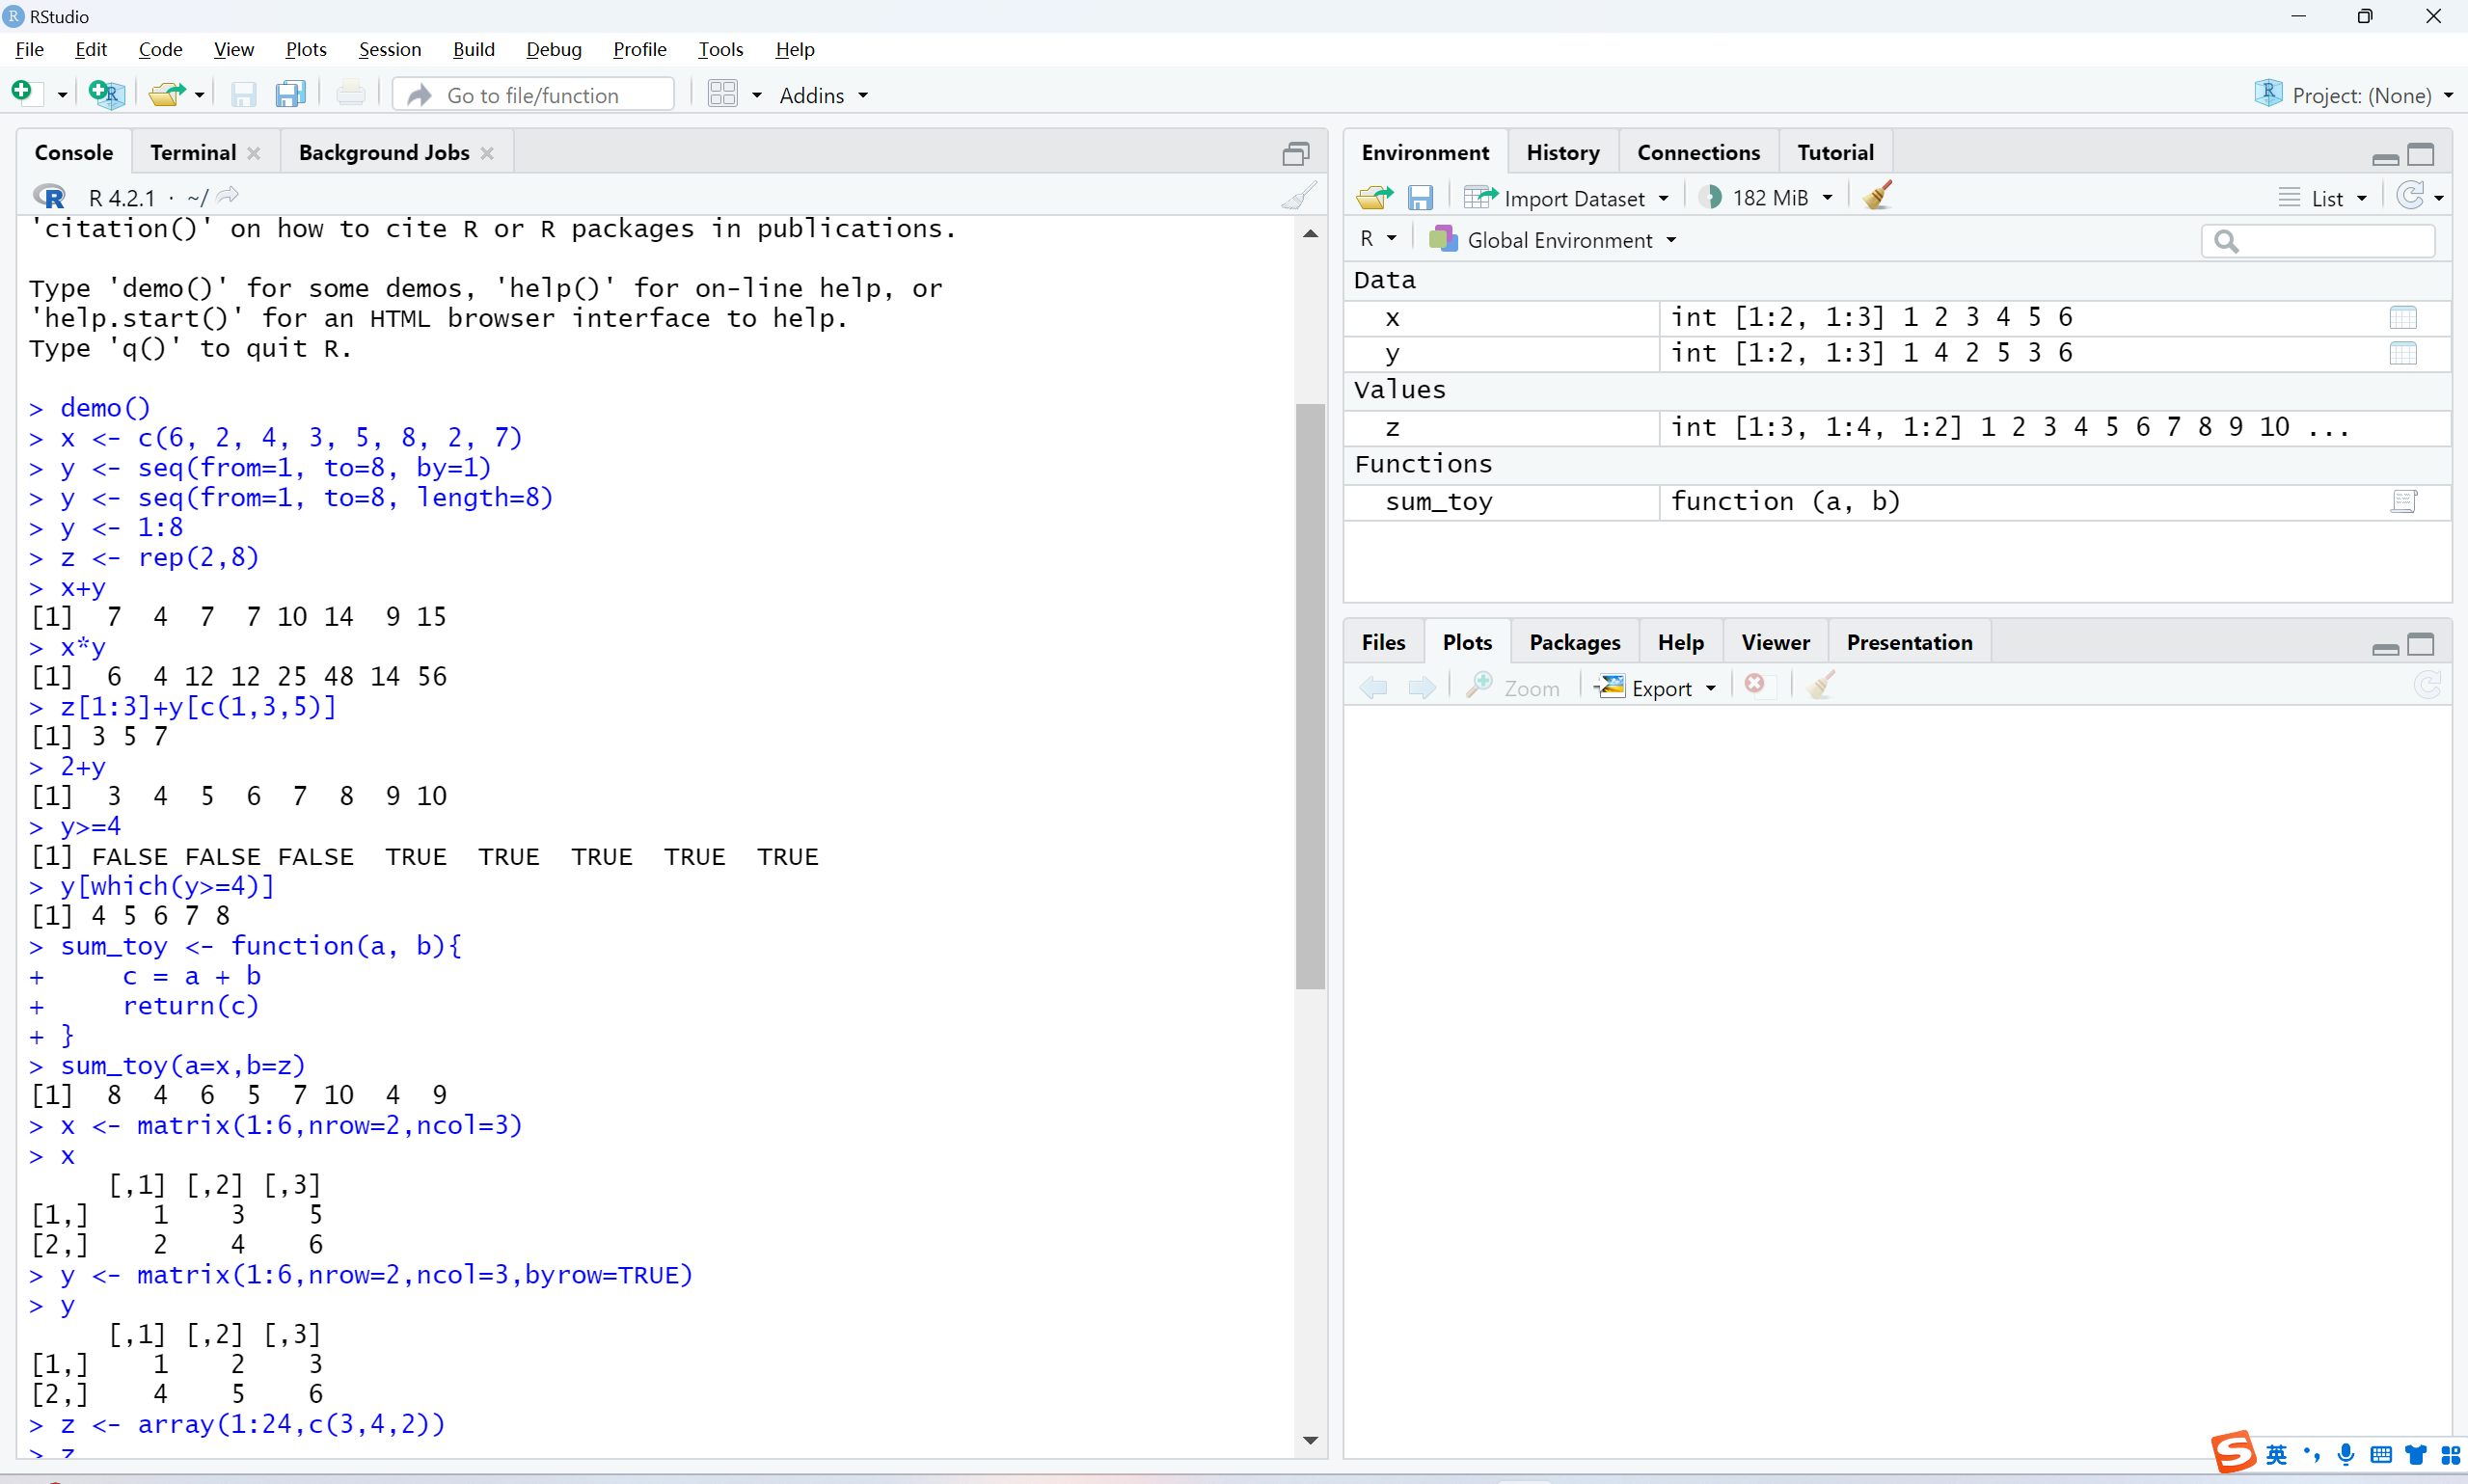
\includegraphics[scale=0.35]{R_test.png}
    \caption{R语言测试}
    \label{1}
    \end{figure}
\end{CJK}
\end{document}